\documentclass[12pt]{article}
\usepackage[margin=0.1in]{geometry}
\usepackage{color}
\usepackage{graphicx}
\usepackage{epstopdf}
\epstopdfsetup{update}
\usepackage{amsmath}
\usepackage{amssymb}
\usepackage[colorlinks]{hyperref}
\usepackage{geometry}
\usepackage[square]{natbib} 

\newcommand{\bea}{\begin{eqnarray}}
\newcommand{\eea}{\end{eqnarray}}
\newcommand{\bF}{\mathbf{F}}
\newcommand{\ba}{\mathbf{a}}
\newcommand{\bA}{\mathbf{A}}
\newcommand{\bu}{\mathbf{u}}
\newcommand{\bg}{\mathbf{g}}
\newcommand{\bB}{\mathbf{B}}
\newcommand{\bd}{\mathbf{d}}
\newcommand{\be}{\mathbf{e}}
\newcommand{\bm}{\mathbf{m}}
\newcommand{\bM}{\mathbf{M}}
\newcommand{\bv}{\mathbf{v}}
\newcommand{\bV}{\mathbf{V}}
\newcommand{\bp}{\mathbf{p}}
\newcommand{\bP}{\mathbf{P}}
\newcommand{\br}{\mathbf{r}}
\newcommand{\bx}{\mathbf{x}}
\newcommand{\bR}{\mathbf{R}}
\newcommand{\bN}{\mathbf{N}}
\newcommand{\bell}{\boldsymbol{\ell}}
\newcommand{\bL}{\mathbf{L}}
\newcommand{\btau}{\boldsymbol{\tau}}
\newcommand{\bT}{\mathbf{T}}
\newcommand{\bi}{\mathbf{i}}
\newcommand{\bj}{\mathbf{j}}
\newcommand{\bk}{\mathbf{k}}
\newcommand{\bn}{\mathbf{n}}
\newcommand{\bomega}{\boldsymbol{\omega}}
\newcommand{\md}{\mathrm{d}}
\newcommand{\ie}{\textit{i.e.{ }}}
\newcommand{\etc}{\textit{etc.{ }}}
\newcommand{\ddt}{\frac{\md}{\md t}}
\newcommand{\ddtt}{\frac{\md^2}{\md t^2}}
\newcommand{\ppt}{\frac{\partial}{\partial t}}
\newcommand{\pptt}{\frac{\partial^2}{\partial t^2}}
\newcommand{\me}{\mathrm{e}}


%===============================================
\begin{document}
\title{Two-points umklapp model}
%\author{Da Wang}%\thanks{dawang@nju.edu.cn} \\ \\National Laboratory of Solid State Microstructures $\&$ School of Physics, \\ Nanjing University, Nanjing, 210093, China}
\date{}
\maketitle

%\begin{abstract}
We are seeking a diagrammatic treatment of the two-points umklapp model. It seems we are doing a trick
\bea \sum_k\int\mathcal{D}\phi \ne \int\mathcal{D}\phi\sum_k \eea
%\end{abstract}

%\tableofcontents
%=================================================
The model is defined as
\bea H=gR_\uparrow^\dag R_\downarrow^\dag L_\downarrow L_\uparrow + h.c. \eea

The partition function is
\bea Z&=&\int{ \mathcal{D}R\mathcal{D}L \me^{\int{ \bar{R}_\sigma (-\partial\tau)R_\sigma + \bar{L}_\sigma (-\partial\tau)L_\sigma -g(\bar{R}_\uparrow \bar{R}_\downarrow L_\downarrow L_\uparrow + h.c.)} }} \\
&=&\int{ \mathcal{D}R\mathcal{D}L \me^{\int {\bar{R}_\sigma (-\partial\tau)R_\sigma + \bar{L}_\sigma (-\partial\tau)L_\sigma +g(\bar{R}_\uparrow \bar{R}_\downarrow-\bar{L}_\uparrow \bar{L}_\downarrow)(R_\downarrow R_\uparrow-L_\downarrow L_\uparrow) - g\bar{R}_\uparrow \bar{R}_\downarrow R_\downarrow R_\uparrow -g \bar{L}_\uparrow \bar{L}_\downarrow L_\downarrow L_\uparrow}}}  \\
&=&\int{ \mathcal{D}R\mathcal{D}L\mathcal{D}\phi \me^{ \int{  \bar{R}_\sigma (-\partial\tau)R_\sigma + \bar{L}_\sigma (-\partial\tau)L_\sigma +[\phi (\bar{R}_\uparrow \bar{R}_\downarrow-\bar{L}_\uparrow \bar{L}_\downarrow) + h.c.]-\frac1g\phi^*\phi  - g\bar{R}_\uparrow \bar{R}_\downarrow R_\downarrow R_\uparrow -g \bar{L}_\uparrow \bar{L}_\downarrow L_\downarrow L_\uparrow }}} \\
&=&\int \mathcal{D}R\mathcal{D}L\mathcal{D}\phi \sum_k \frac{(-g)^k}{k!} \int \md^k\tau \mathcal{T}_\tau (\bar{R}_\uparrow \bar{R}_\downarrow R_\downarrow R_\uparrow +\bar{L}_\uparrow \bar{L}_\downarrow L_\downarrow L_\uparrow)^k \nonumber\\ 
&&  \me^{ \int{  \bar{R}_\sigma (-\partial\tau)R_\sigma + \bar{L}_\sigma (-\partial\tau)L_\sigma +[\phi (\bar{R}_\uparrow \bar{R}_\downarrow-\bar{L}_\uparrow \bar{L}_\downarrow) + h.c.]-\frac1g\phi^*\phi  }} \\
&\rightarrow&\int \mathcal{D}\phi\sum_k\frac{(-g)^k}{k!}\int \md^k\tau\mathcal{T}_\tau(\partial_{\eta_\uparrow}\partial_{\eta_\downarrow}\partial_{\bar{\eta}_\downarrow}\partial_{\bar{\eta}_\uparrow}+\partial_{\xi_\uparrow}\partial_{\xi_\downarrow}\partial_{\bar{\xi}_\downarrow}\partial_{\bar{\xi}_\uparrow})^k \nonumber\\&& \me^{\mathrm{Tr}\log(\partial_\tau+\hat{\phi})+\mathrm{Tr}\log(\partial_\tau-\hat{\phi})+\bar{\eta}(\partial_\tau+\hat{\phi})^{-1}\eta+\bar{\xi}(\partial_\tau-\hat{\phi})^{-1}\xi-\frac1g\phi^*\phi} \\
&=& \int \mathcal{D}\phi \sum_k \frac{(-g)^k}{k!}\int \md^k\tau \mathcal{T}_\tau (\partial_{\eta_\uparrow}\partial_{\eta_\downarrow}\partial_{\bar{\eta}_\downarrow}\partial_{\bar{\eta}_\uparrow}+\partial_{\xi_\uparrow}\partial_{\xi_\downarrow}\partial_{\bar{\xi}_\downarrow}\partial_{\bar{\xi}_\uparrow})^k \me^{S[\phi,\eta,\xi]} \eea
where we have introduced the source $\eta$ and $\xi$ coupled to $R$ and $L$, respectively. 
The exact Green's function $G_R$ is given by
\bea \hat{G}_R&=&\frac{1}{Z}\int \mathcal{D}\phi \sum_k \frac{(-g)^k}{k!} \int\md^k\tau\mathcal{T}_\tau \partial_{\bar{\eta}} \partial_\eta (\partial_{\eta_\uparrow}\partial_{\eta_\downarrow}\partial_{\bar{\eta}_\downarrow}\partial_{\bar{\eta}_\uparrow}+\partial_{\xi_\uparrow}\partial_{\xi_\downarrow}\partial_{\bar{\xi}_\downarrow}\partial_{\bar{\xi}_\uparrow})^k \me^{S[\phi,\eta,\xi]} \\
&=&\frac{\int\mathcal{D}\phi \left[\sum {\rm connected}\right]_\phi\left[\sum {\rm closed}\right]_\phi \me^{S[\phi]} }{\int\mathcal{D}\phi \left[\sum {\rm closed}\right]_\phi \me^{S[\phi]}}
\eea
Clearly, if without $\phi$, the closed diagrams can be canceled. But when $\phi$ exists, we cannot do such a simplification unless $|\phi|$ is pinned at a fixed value like in $T=\infty$ and $T=0$ limits. The former is just the usual diagrammatic expansion while the latter is the mean field theory. 

Next, let us seek an (semi-)analytical treatment. Let's first try the approximation of $\phi(\tau)=\phi$, \ie time independent. Then, $\int \mathcal{D}\phi\rightarrow\int\md\phi$ and
\bea S(\phi)=2\log(1+\me^{-\beta|\phi|})+2\log(1+\me^{\beta|\phi|})-\frac{\beta|\phi|^2}{g} \eea  

A second approximation is to truncate $k$ with a upper bound $N_k$. When $N_k=0$, we have omitted all closed diagrams, \ie $\sum[{\rm closed}]=1$. Then, we have
\bea G_R=\left. \int\md \phi \frac{1}{2}\left(\frac{1}{i\omega_n-|\phi|}+\frac{1}{i\omega_n+|\phi|}\right) \me^{S(\phi)}  \middle/ \int\md  \phi \me^{S(\phi)}\right. \eea

Next, let's set $N_k=1$. However, the result becomes worse. The reason is the amplitude fluctuations can not be neglected in the middle temperature regime.  
\begin{figure}[h]
    \begin{center}
    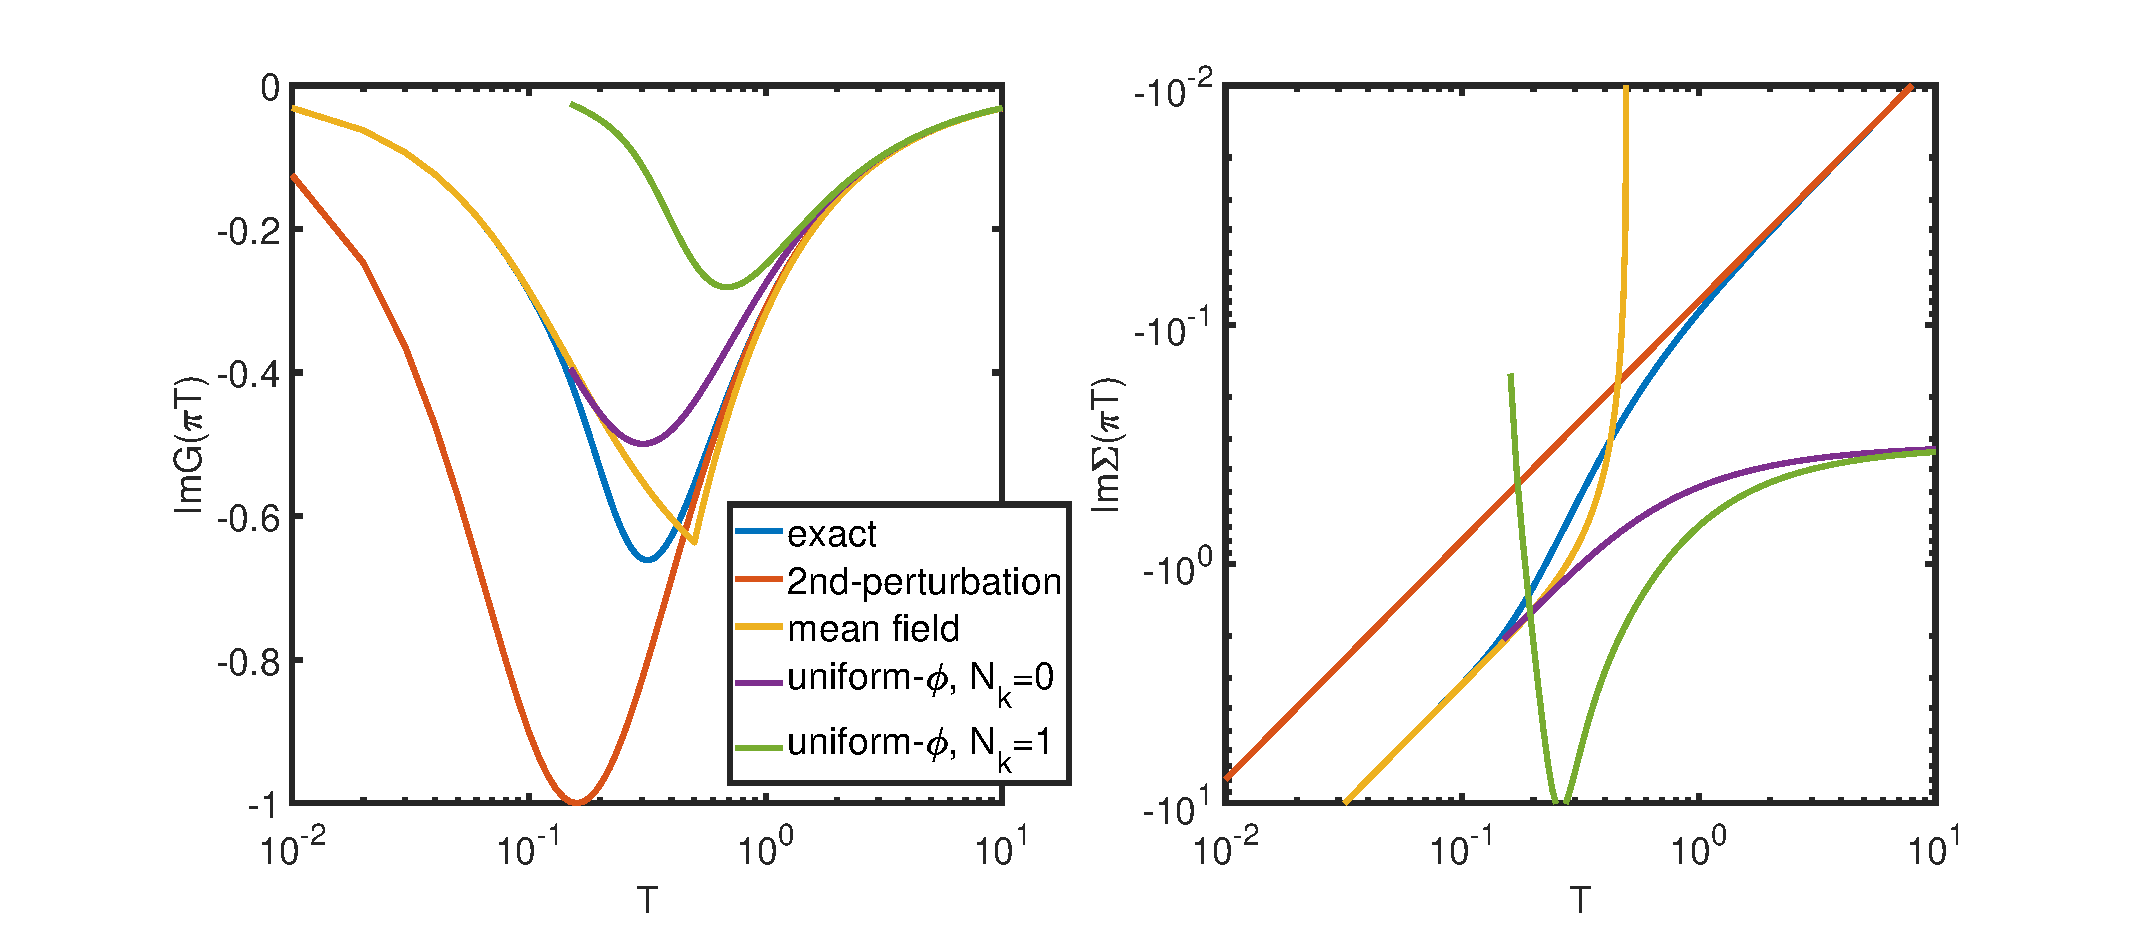
\includegraphics[width=0.8\textwidth]{result.eps}
    \caption{Approximation of time-independent $\phi$.}
    \end{center}
\end{figure}

When $\phi$ depends on $\tau$, or equivalently $i\nu_n\ne0$, the bare Green's function under a given $\phi$ depends on two frequencies and can be written as
\bea G_{0R}^{-1}(i\omega_n,i\omega_n')=i\omega_n\delta(\omega_n-\omega_n')-\phi(i\omega_n-i\omega_n')\sigma_+-\phi^*(i\omega_n-i\omega_n')\sigma_- \eea
and
\bea G_{0L}^{-1}(i\omega_n,i\omega_n')=i\omega_n\delta(\omega_n-\omega_n')+\phi(i\omega_n-i\omega_n')\sigma_++\phi^*(i\omega_n-i\omega_n')\sigma_- \eea
Now the bare action $S[\phi]$ becomes
\bea S[\phi]=\mathrm{Tr}\log(\partial_\tau+\hat{\phi})+\mathrm{Tr}\log(\partial_\tau-\hat{\phi})-\frac{T}{g} \sum_{i\nu_n}|\phi(\nu_n)|^2=S_0[\phi_0]+\delta S[\phi_0,\delta\phi] \eea
where $\phi=\phi_0+\delta\phi$ with $\phi_0$ the uniform field. One reasonable(?) approximation is to suppose $\delta\phi$ much smaller than $\phi_0$ such that we can expand $\delta S$ with respect to $\delta\phi$ up to the second order. (Higher order expansions can be performed but difficult to integrate out.) 
\bea \delta S=-\frac12\sum_{R,L}\mathrm{Tr}(G_0^{R,L}\delta\phi G_0^{R,L} \delta\phi)  -\frac{T}{g}\sum_{\nu_0\ne0}\phi^*(\nu_n)\phi(\nu_n) \eea
where $G_0^{R,L}$ are the bare Green's function under the uniform $\phi_0$. Notice that $G_0^{R,L}$ and $\delta\phi$ are both matrices. The source terms can also be expand with respect to $\delta\phi$. Put the above together, we have
\bea S&=&2\log(1+\me^{-\beta|\phi_0|})+2\log(1+\me^{\beta|\phi_0|})-\frac{\beta|\phi_0|^2}{g}\nonumber\\
&& -\frac12\mathrm{Tr}(G_0^{R}\delta\phi G_0^{R} \delta\phi) -\frac12\mathrm{Tr}(G_0^{L}\delta\phi G_0^{L} \delta\phi) -\frac{T}{g}\sum_{\nu_0\ne0}\phi^*(\nu_n)\phi(\nu_n) \nonumber\\&&-\bar{\eta}(G_0^R+G_0^R\delta\phi G_0^R+G_0^R\delta\phi G_0^R\delta\phi G_0^R+\cdots)\eta \nonumber\\&&-\bar{\xi}(G_0^L-G_0^L\delta\phi G_0^L+G_0^L\delta\phi G_0^L\delta\phi G_0^L+\cdots)\xi \eea
Notice that at this step, we cannot trace out $\delta\phi$ directly otherwise the source terms would become too complicated.

\bea &&\mathrm{Tr}(G_0^R\delta\phi G_0^R\delta\phi)\nonumber\\&=&T^2\sum_{i\nu_n,i\omega_n}\left[G_{11}^R(i\omega_n)G_{22}^R(i\omega_n+i\nu_n)\phi^*(\nu_n)\phi(\nu_n)+G_{22}^R(i\omega_n)G_{11}^R(i\omega_n+i\nu_n)\phi^*(-\nu_n)\phi(-\nu_n) \right. \nonumber\\
&&\left.+G_{12}^R(i\omega_n)G_{12}^R(i\omega_n+i\nu_n)\phi^*(\nu_n)\phi^*(-\nu_n)+G_{21}^R(i\omega_n)G_{21}^R(i\omega_n+i\nu_n)\phi(\nu_n)\phi(-\nu_n)\right] \nonumber\\
&=&-T\sum_{i\nu_n}\frac{|\phi_0|}{\nu_n^2+4|\phi_0|^2}\tanh\left(\frac{\beta|\phi_0|}{2}\right)\left[\phi^*(\nu_n)\phi(\nu_n)+\phi^*(-\nu_n)\phi(-\nu_n)-\frac{\phi_0^2}{|\phi_0|^2}\phi^*(\nu_n)\phi^*(-\nu_n)-\frac{\phi_0^{*2}}{|\phi_0|^2}\phi(\nu_n)\phi(-\nu_n)\right]\nonumber \\
&=& \mathrm{Tr}(G_0^L\delta\phi G_0^L\delta\phi)
\eea

Then \bea \delta S&=&T\sum_{\nu_n\ne0}\frac{|\phi_0|}{\nu_n^2+4|\phi_0|^2}\tanh\left(\frac{\beta|\phi_0|}{2}\right)\left[\phi^*(\nu_n)\phi(\nu_n)+\phi^*(-\nu_n)\phi(-\nu_n)-\frac{\phi_0^2}{|\phi_0|^2}\phi^*(\nu_n)\phi^*(-\nu_n)-\frac{\phi_0^{*2}}{|\phi_0|^2}\phi(\nu_n)\phi(-\nu_n)\right] \nonumber\\ &&- \frac{T}{g}\sum_{\nu_n\ne0}\phi^*(\nu_n)\phi(\nu_n) \nonumber\\
&=&-\sum_{\nu_n>0}\begin{bmatrix}
    \phi^*(\nu_n) & \phi(-\nu_n)
\end{bmatrix}\begin{bmatrix}
\frac{T}{g}-\frac{2T|\phi_0|\tanh(\beta|\phi_0|/2)}{\nu_n^2+4|\phi_0|^2} & \frac{\phi_0^2}{|\phi_0|^2}\frac{2T|\phi_0|\tanh(\beta|\phi_0|/2)}{\nu_n^2+4|\phi_0|^2} \\ \frac{\phi_0^{*2}}{|\phi_0|^2}\frac{2T|\phi_0|\tanh(\beta|\phi_0|/2)}{\nu_n^2+4|\phi_0|^2} & \frac{T}{g}-\frac{2T|\phi_0|\tanh(\beta|\phi_0|/2)}{\nu_n^2+4|\phi_0|^2}
\end{bmatrix} \begin{bmatrix}
\phi(\nu_n) \\ \phi^*(-\nu_n)
\end{bmatrix}\eea


When $N_k=0$, $[closed]=1$ and 
\bea [connected]=G_0^R+G_0^R\delta\phi G_0^R+G_0^R\delta\phi G_0^R\delta\phi G_0^R+\cdots \eea
The first order will vanish. Higher orders are omitted. We then have
\bea [connected]_{R11}&=&G_0^R+G_0^R\delta\phi G_0^R\delta\phi G_0^R \nonumber\\
&=&G_{11}^R(i\omega_n)+T\sum_{i\nu_n}G_{11}(i\omega_n)\phi(\nu_n)G_{21}(i\omega_n+i\nu_n)\phi(-\nu_n)G_{21}(i\omega_n) \nonumber\\
&& + G_{11}(i\omega_n)\phi(\nu_n)G_{22}(i\omega_n+i\nu_n)\phi^*(\nu_n)G_{11}(i\omega_n) \nonumber\\
&& + G_{12}(i\omega_n)\phi^*(-\nu_n)G_{11}(i\omega_n+i\nu_n)\phi(-\nu_n)G_{21}(i\omega_n) \nonumber\\
&& + G_{12}(i\omega_n)\phi^*(-\nu_n)G_{12}(i\omega_n+i\nu_n)\phi^*(\nu_n)G_{11}(i\omega_n) \nonumber\\
&=& G_{11}^R(i\omega_n) + T\sum_{\nu_n>0}\begin{bmatrix}
    \phi^*(\nu_n) & \phi(-\nu_n)
\end{bmatrix}\begin{bmatrix}
a & b\\c &d
\end{bmatrix} \begin{bmatrix}
\phi(\nu_n) \\ \phi^*(-\nu_n)
\end{bmatrix}
\eea
where 
\bea a=G_{11}(i\omega_n)G_{22}(i\omega_n+i\nu_n)G_{11}(i\omega_n)+G_{12}(i\omega_n)G_{11}(i\omega_n-i\nu_n)G_{21}(i\omega_n) \eea
\bea b=G_{12}(i\omega_n)G_{12}(i\omega_n+i\nu_n)G_{12}(i\omega_n)+G_{12}(i\omega_n)G_{12}(i\omega_n-i\nu_n)G_{12}(i\omega_n) \eea
\bea c=G_{11}(i\omega_n)G_{21}(i\omega_n+i\nu_n)G_{21}(i\omega_n)+G_{11}(i\omega_n)G_{21}(i\omega_n-i\nu_n)G_{21}(i\omega_n) \eea
\bea d=G_{12}(i\omega_n)G_{11}(i\omega_n+i\nu_n)G_{21}(i\omega_n)+G_{11}(i\omega_n)G_{22}(i\omega_n-i\nu_n)G_{11}(i\omega_n) \eea

Using the identity
\bea \int \md X^* \md X (A_0+X^\dag A_2 X)\me^{-X^\dag D X}=\det(D)^{-1}[A_0+{\rm tr}(A_2D^{-1})] \eea
we can trace out $\delta\phi$. {\color{red} Notice: $\det(D)$ can be negative under a given $\phi_0$ in which case, we need to use $|\det{D}|$ as the weight and $-G$ as the measurable just like what we do in QMC.}

We fail again! When $\det(D)$ is very small, the fluctuation of $\delta\phi$ can be very strong so as to break the perturbation condition!



\bibliography{bibfile}
%\begin{thebibliography}{99}
%	\bibitem{xxxx} xxxx, PRL 88, 888888 (2088).
%\end{thebibliography}
\end{document}
